\documentclass[10pt,a4paper]{article}

\usepackage[utf8]{inputenc}
\usepackage[T1]{fontenc}
\usepackage[italian]{babel}
\usepackage{graphicx}
\usepackage{amsmath,amssymb,amsfonts}
\usepackage{caption}
\usepackage{subcaption}
\usepackage{wrapfig}
\usepackage{float}
\usepackage{geometry}
\geometry{top=2.5cm, bottom=2.5cm, left=1.7cm, right=1.7cm}
\usepackage{fancyhdr}
\usepackage{titlesec}
\usepackage{lmodern}
\usepackage{caption}
\usepackage{comment}
\usepackage{booktabs}
\usepackage{makecell}
\usepackage{siunitx}
\usepackage{bm}
\usepackage[version=4]{mhchem} 
\DeclareCaptionFont{myit}{\footnotesize\itshape\fontfamily{cmr}\selectfont}
\captionsetup{
    font=myit,
    labelfont={bf},
    textfont=normalfont
}
\usepackage{titletoc}

% Intestazioni moderne
\pagestyle{fancy}
\fancyhf{}
\fancyhead[L]{Vita media del $\mu$}
\fancyhead[R]{Niccolò Menichetti \\ Luca Musetti \\ Luca Nasone}
\fancyfoot[C]{\thepage}

% Re e Im
\renewcommand{\Re}{\mathop{\mathrm{Re}}}
\renewcommand{\Im}{\mathop{\mathrm{Im}}}

% Per "simulare" capitoli
\newcommand{\chapter}[1]{
    \clearpage
    \section*{#1}
    \addcontentsline{toc}{section}{#1}
}

\title{\bfseries Relazione di laboratorio \\[1ex] \Large Vita media del $\mu$}
\author{Niccolò Menichetti \\ Luca Musetti \\ Luca Nasone}
\date{Anno Accademico 2025--2026}

\begin{document}

\begin{titlepage}
    \thispagestyle{empty}
    
    \begin{figure}[ht]
        \centering
        \begin{minipage}{0.48\textwidth}
            \centering
            
\includegraphics[width=5.0cm]{Immagini/Stemma_unipi.svg.png}
        \end{minipage}%
        \hfill
        \begin{minipage}{0.48\textwidth}
            \centering
            
\includegraphics[width=7.0cm]{Immagini/unipi_fermi.png}
        \end{minipage}
    \end{figure}

    \vspace{4.0cm} % Spazio per centrare verticalmente il contenuto

    \begin{center}
        {\fontsize{20pt}{24pt}\selectfont\bfseries Vita media del muone}\\[0.3cm]
        {\large Relazione laboratorio di interazioni fondamentali}\\[9.0cm]

        {\Large NICCOLO' MENICHETTI\hspace{0.2cm} LUCA MUSETTI \hspace{0.2cm} LUCA NASONE}\\[0.35cm]
        {\normalsize Anno Accademico 2025 - 2026}
    \end{center}

\end{titlepage}

\newpage

\begin{abstract}
        
    \emph{Nella seguente relazione descriviamo la nostra misura della vita media del muone, effettuata sui muoni dei raggi cosmici. Otteniamo una vita media pari a $2.123\pm 0.035$ $\mu$s...(to be continued)}
        
\end{abstract}

\tableofcontents

\newpage

\section{Introduzione}

\begin{flushleft}
Sappiamo che, a causa dell'interazione con l'atmosfera, i raggi cosmici che arrivano dallo spazio hanno una composizione differente a livello del mare. In particolare prevalgono i muoni $\mu$, che decadono nel seguente modo:

\begin{equation}\label{mu_decay}
    \ce{$\mu^{-}\rightarrow e^{-}\bar \nu_e \nu_{\mu}$}
\end{equation}

con vita media è $\tau_{\mu} = 2.1969811 \pm 0.0000022 $ $\mu s$ (PDG 2025) e carica $\pm e$.

L'obiettivo dell'esperimento è misurare il valore della vita media del muone, con un apparato sperimentale in grado di rilevare i raggi cosmici e fermare i $\mu$ a bassa energia. 

Nella materia i muoni negativi tendono a formare degli stati legati con i nuclei (atomi mesici). Questo fatto rende la vita media del muone con carica negativa più bassa di quella per muoni con carica positiva. Con i dati a nostra disposizione possiamo estrarre l'abbondanza relativa di una specie rispetto all'altra, ossia $N_+/N_-$, note le popolazioni $N_+$ e $N_-$ per i muoni con la carica $\pm e$ rispettivamente.

Utilizzando gli impulsi rilasciati nei fotomoltiplicatori, è stato possibile, previa un'opportuna calibrazione, misurare lo spettro in energia dell'$e^{-}$ prodotto dal decadimento. Essendo un decadimento a 3 corpi che sappiamo che per certo non essere monocromatico, in approssimazione di $m_{\nu} \simeq 0 $ $ m_\mu \gg m_e $ si ricava facilmente dalla cinematica relativistica il limite superiore:

\begin{equation}\label{E_max}
    (E_e)^{max} = \frac{m_{\mu}^2+m_{e}^2}{2m_{\mu}} \approx \frac{m_\mu}{2}
\end{equation}



Usando $m_\mu = 105.6583755 \pm 0.0000023\text{MeV}$\footnote{PDG 2025}, si ottiene  $(E_e)^{max} =52.82918775 \pm 0.00000011 \text{MeV}$. 
Dalla relazione \ref{E_max} è possibile ottenere una stima della massa del $\mu$ ricostruendo la distribuzione in energia degli elettroni di decadimento e individuando il valore di energia dove si osserva un limite superiore.

\end{flushleft}
\newpage

\section{Apparato sperimentale}

\begin{figure}[h]
\centering
\begin{minipage}{0.40\textwidth}
    \centering
    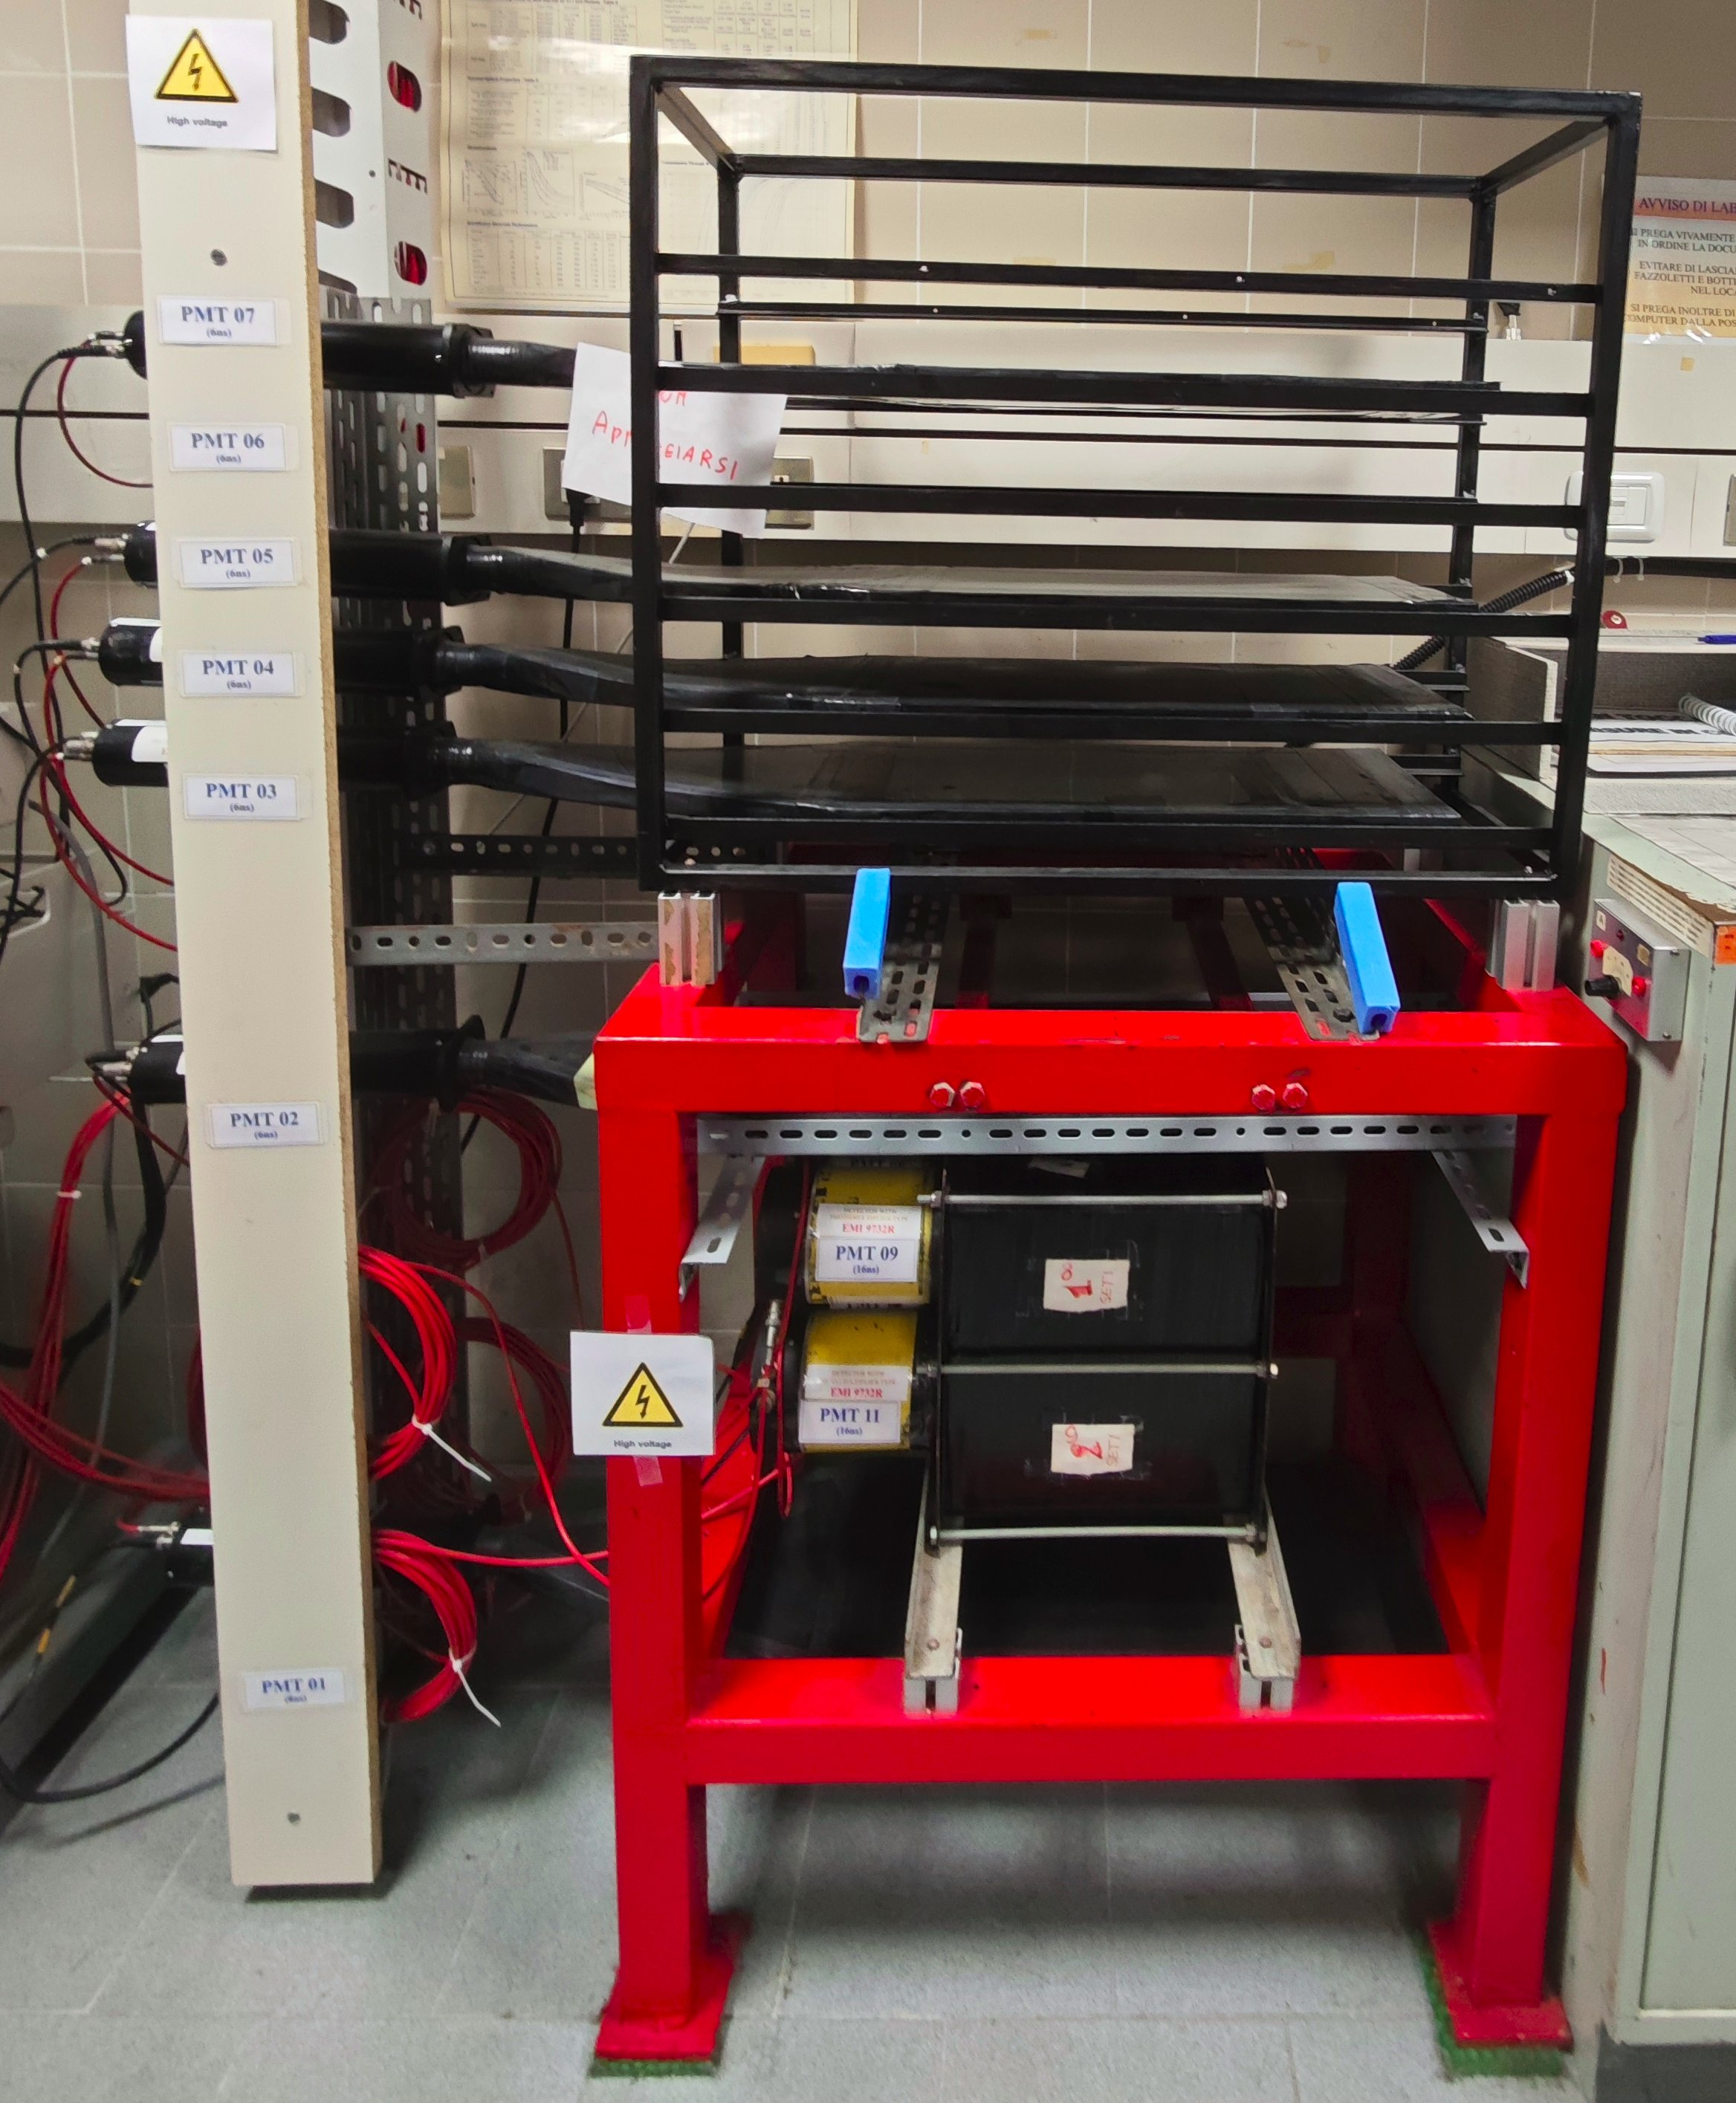
\includegraphics[width = 0.85\textwidth]{Immagini/apparato1.jpg}
    \label{telescopio}
    \caption{Scintillaotri e PMT a disposizione}
\end{minipage}
\begin{minipage}{0.4\textwidth}
    \centering
    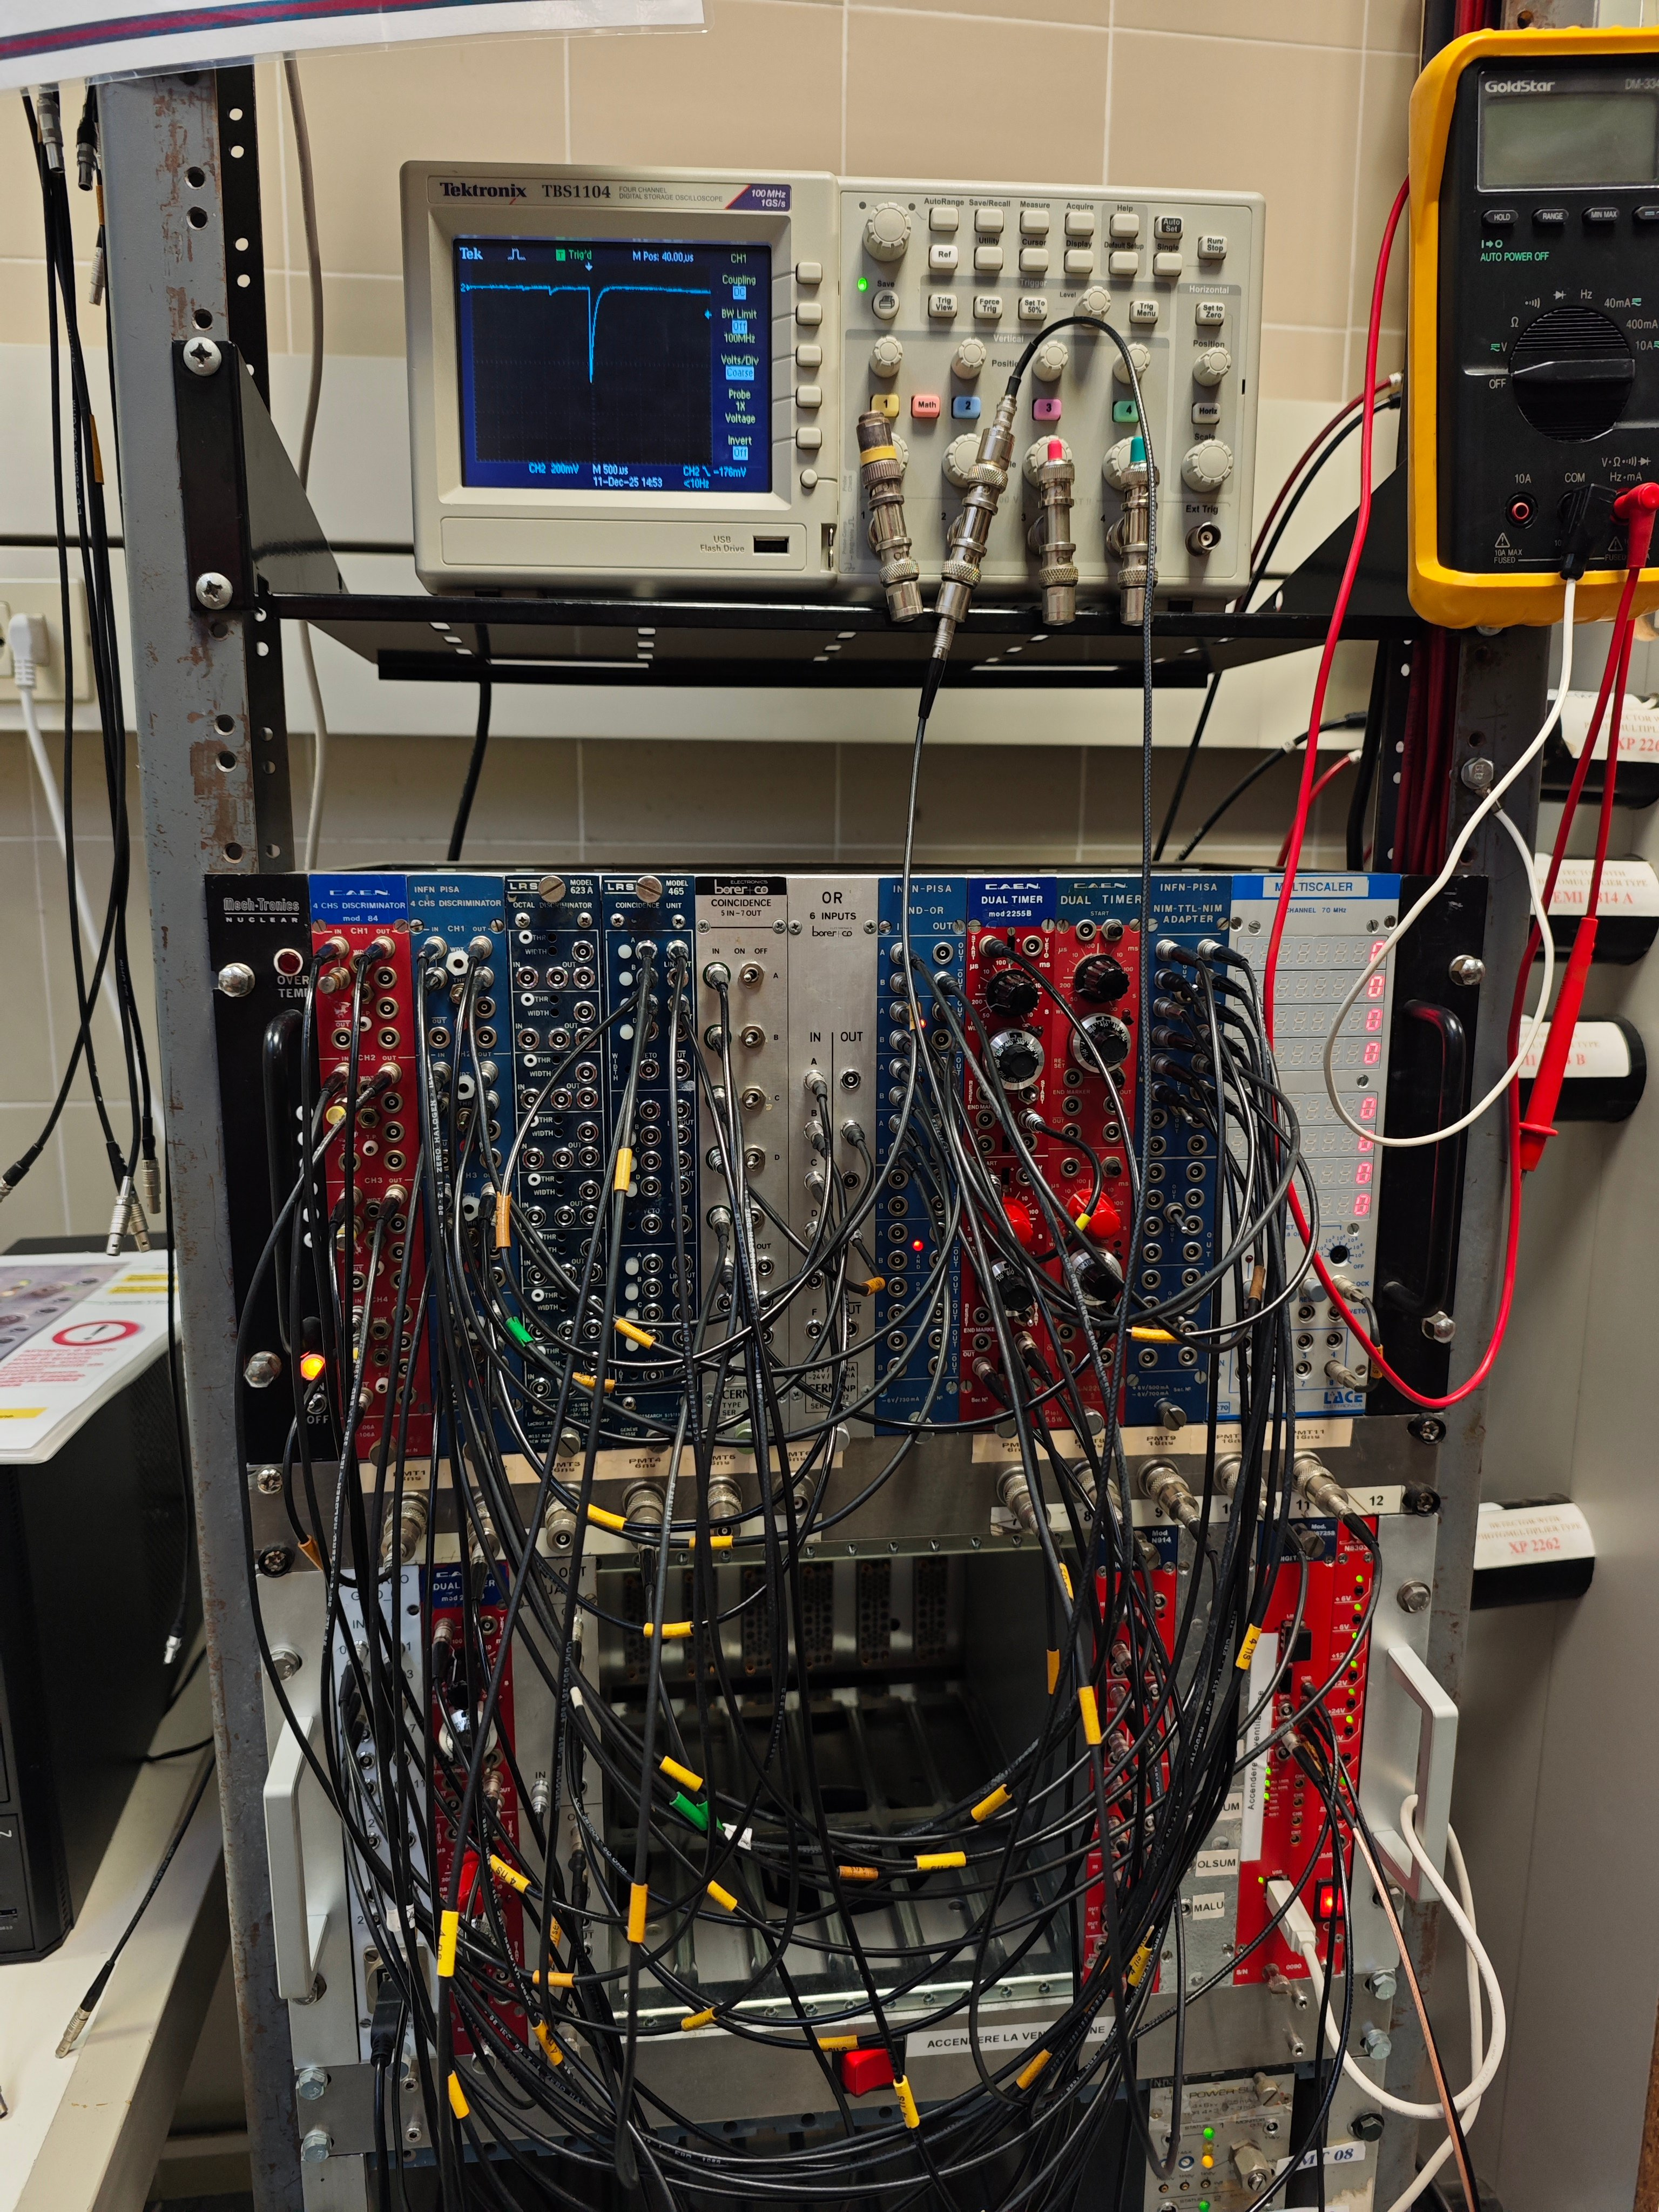
\includegraphics[width = 0.85\textwidth]{Immagini/moduli1.jpg}
    \label{rack}
    \caption{Rack con alcuni moduli utilizzati}
\end{minipage}
\end{figure}
Gli strumenti utilizzati nel corso dell'esperienza sono:
\begin{itemize}
\item Alimentatore alto voltaggio ....
\item 6 lastre di scintillatore a disposizione per il telescopio ((49.8 $\pm$ 0.1 cm) $\times$ (27.5 $\pm$ 0.1 cm) $\times$ (2.3 $\pm$ 0.1 cm)), collegate ciascuna a un fotomoltiplicatore (PMT 1-2-3-4-); 
\item 1 blocco di scintillatore dimensioni (30.0 $\pm$ 0.1 cm) $\times$ (31.0 $\pm$ 0.1 cm) $\times$ (31.0 $\pm$ 0.1), collegato a 4 PMT; 
\item una scheda di sviluppo con FPGA DE0-10 NANO;
\item 2 discriminatori (NIM CAEN N84 e NIM INFN);
\item 3 unità di coincidenza (NIM LRS 465, NIM CERN N6234, NIM);
\item 1 unità di OR (NIM CERN);
\item 2 unità di Dual Timer (NIM CAEN mod2255B e NIM CAEN N2255);
\item 1 unità di conversione NIM-TTL;
\item 1 multiscaler (NIM INFN Multiscaler130);
\item 1 unità di Fan-Out;
\item 1 integratore analogico (NIM CAEN N914);
\item 1 ADC (NIM CAEN N6725);
\item 1 oscilloscopio;
\item 2 computer, per regolare le alimentazioni e per le acquisizioni;
\item 1 multimetro digitale;
\item cavi coassiali di vario ritardo e terminazioni a 50 e 0 $\Omega$;
\item 1 metro a nastro;
\end{itemize}

\section{Punto di lavoro}

\subsection{Telescopio}
\begin{flushleft}
La prima attività svolta è stato scegliere il punto di lavoro dei vari PMT. Soglie e alimentazioni influenzano l'efficienza e di conseguenza il numero di eventi rivelati. Vogliamo sia più alta possibile in modo da massimizzare la statistica a nostra disposizione. 

Dopo una fase di test in cui abbiamo osservato il rate in singola dei vari PMT, sono stati scelti il PMT07, il PMT04 e il PMT02. Come stima dell'efficienza di un PMT (poniamo ad esempio il PMT07) abbiamo usato il rapporto fra le coincidenze triple $(07\land04\land02)$ e le coincidenze doppie degli altri due (nel nostro esempio $(04\&02)$). 

Misuriamo i conteggi combinando i segnali discriminati tramite le unità di coincidenza, le cui uscite sono in seguito inviate al multiscaler, che conta per 100 s. La misura viene poi ripetuta variando l'alimentazione.

Durante la procedura sono state misurate anche le singole dei due PMT usati per le coincidenze doppie, in quanto il loro rate in singola influenza il rate delle doppie false, ottenuto da:
\begin{equation}
    \label{fake}
    D_{fake} = R_1 R_2 (w_1 + w_2 - 2w)
\end{equation}

Dove $R_1$ e $R_2$ sono i rate in singola dei PMT di interesse, $w_1$ e $w_2$ sono le durate dei loro segnali discriminati (50 ns nel nostro caso). $w$ è la sovrapposizione temporale minima per avere una coincidenza, di 2 ns. Sceglieremo alimentazioni e soglie cercando di rendere il numero di doppie false trascurabile rispetto alle doppie misurate.


Tale procedura è ottimale per il PMT04, ma non per il PMT07 e PMT02, a causa della geometria del sistema. 
Per correggere tale effetto abbiamo usato un metodo Montecarlo per simulare il passaggio dei raggi cosmici attraverso il rivelatore, al fine di ricavare la probabilità che un raggio cosmico passi per un PMT dato il passaggio dagli altri due (accettanza). 
Dividendo il rapporto triple su doppie misurato con tale valore si ottiene una stima dell'efficienza.

Stimiamo l'errore sul rapporto triple su doppie con: 

\begin{equation}
    \label{error_eff}
    \sigma_{\varepsilon} = \sqrt{\frac{\varepsilon(1-\varepsilon)}{D}}
\end{equation}

dove $D$ è il numero di doppie.


Riportiamo le misure fatte nelle tabelle sottostanti, le colonne sono voltaggio di alimentazione, efficienza, errore sull'efficienza e numero di doppie fake, con il titolo che si riferisce al PMT per cui si sono eseguite le misure:

\begin{table}[H]
    \begin{minipage}{0.3\linewidth}
        \centering
        \resizebox{1\linewidth}{!}{    \begin{tabular}{cccc}
    \toprule
    $HV$[V] ($\pm$ 1V) & $\varepsilon$ [$\%$] & $\sigma_{\varepsilon}$[$\%$] & $D_{fake}$ \\
    \midrule
    1675 & 52 & $\pm$ 2 & 0.69 \\
    1700 & 70 & $\pm$ 2 & 0.65 \\
    1720 & 80 & $\pm$ 1 & 0.63 \\
    1730 & 81 & $\pm$ 1 & 0.59 \\
    1750 & 89 & $\pm$ 1 & 0.53 \\
    1775 & 80 & $\pm$ 1 & 0.54 \\
    1800 & 91 & $\pm$ 1 & 0.56 \\
    \bottomrule
    \end{tabular}}
        \caption{PMT02}
        \label{tab:PMT02}
    \end{minipage}
    \hfill
    \begin{minipage}{0.3\linewidth}
        \centering
        \resizebox{1\linewidth}{!}{    \begin{tabular}{cccc}
    \toprule
    $HV$[V] ($\pm$ 1V)& $\varepsilon$ [$\%$] & $\sigma_{\varepsilon}$[$\%$] & $D_{fake}$ \\
    \midrule
    1675 & 87 & $\pm$ 2 & 0.077 \\
    1700 & 94 & $\pm$ 1 & 0.068 \\
    1720 & 94 & $\pm$ 1 & 0.074 \\
    1730 & 92 & $\pm$ 2 & 0.073 \\
    1750 & 93 & $\pm$ 1 & 0.078 \\
    1775 & 94 & $\pm$ 1 & 0.076 \\
    1800 & 92 & $\pm$ 1 & 0.076 \\
    \bottomrule
    \end{tabular}}
        \caption{PMT04}
        \label{tab:PMT04}
    \end{minipage}
    \hfill
\begin{minipage}{0.3\linewidth}
        \centering
        \resizebox{1\linewidth}{!}{    \begin{tabular}{cccc}
    \toprule
    $HV$[kV] ($\pm$ 1V)& $\varepsilon$ [$\%$] & $\sigma_{\varepsilon}$[$\%$] & $D_{fake}$ \\
    \midrule
    1.675 & 50 & $\pm$ 2 & 0.97 \\
    1.700 & 77 & $\pm$ 2 & 0.79 \\
    1.720 & 83 & $\pm$ 1 & 0.73 \\
    1.730 & 78 & $\pm$ 2 & 0.73 \\
    1.750 & 80 & $\pm$ 2 & 0.68 \\
    1.775 & 92 & $\pm$ 1 & 0.64 \\
    1.800 & 88 & $\pm$ 1 & 0.57 \\
    \bottomrule
    \end{tabular}}
        \caption{PMT07}
        \label{tab:PMT07}
    \end{minipage}
\end{table}

\begin{figure}[H]
    \label{Eff_curv_telescope}
    \centering
    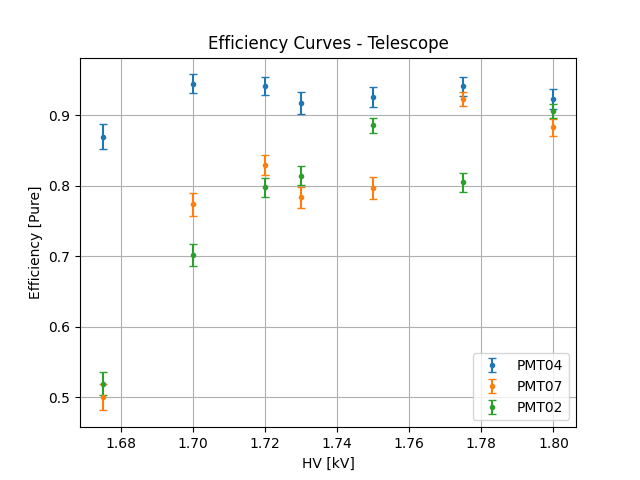
\includegraphics[width = 0.45\textwidth]{Grafici/Efficiency Curves - Telescope.png}
    \caption{Grafico delle curve di efficenza per i PMT02-04-07}
\end{figure}


\begin{table}[H]
    \begin{minipage}{0.5\linewidth}
         In conclusione il punto di lavoro scelto per il telescopio è:
    \end{minipage}
    \begin{minipage}{0.5\linewidth}
        \centering
        \resizebox{1\linewidth}{!}{\begin{tabular}{cccc}
\toprule
Parametro & PMT02 & PMT04 & PMT07 \\
\midrule
$V_{supply}$ [V] & 1750 & 1700 & 1750 \\
$V_{thr}$ [mV] & -30 & -30 & -30 \\
$\varepsilon$ [$\%$] & 88 & 94 & 79 \\
\bottomrule
\end{tabular}}
        \caption{Punto di lavoro scelto per i PMT del telescopio}
        \label{tab:work_scope}              
    \end{minipage}
\end{table}


\end{flushleft}


\subsection{Bersaglio}

\begin{flushleft}
    
Abbiamo ricostruito la curva di efficienza anche per i PMT del bersaglio. 
Al fine di creare una geometria favorevole alla misura, abbiamo usato diverse combinazioni di scintillatori in modo che il rivelatore del quale si misurava l'efficienza risultasse posizionato in mezzo agli altri due.
Abbiamo fatto uno studio analogo per il bersaglio, in questo caso, al fine di creare una geometria favorevole alla misura di efficienza, abbiamo variato gli scintillatori usati, riportiamo le combinazioni usate per ciascun PMT del blocco:

\begin{itemize}

\item PMT08 : PMT02-PMT08-PMT10 
\item PMT09 : PMT02-PMT09-PMT01
\item PMT10 : PMT07-PMT08-PMT10
\item PMT11 : PMT09-PMT11-PMT01

\end{itemize}

Per PMT08-09-11 si è usato il metodo dei trigger ortogonali con lo scintillatore immediatamente sopra/sotto.
Può sicuramente sembrare insolito il PMT10, la ragione è che esso è fuori asse col PMT01, quindi non ci è sembrato ragionevole usarlo. Invece usando il PMT08 (immediatamente sopra) e il PMT07 (il più in alto di tutti) abbiamo pensato potesse stringere opportunamente l'angolo solido, in modo da aumentare l'accettanza e dunque avere una stima più veritiera dell'efficienza partendo dal rapporto triple su doppie. 
Per il resto, le misure di rate si sono svolte come descritto nella sezione precedente, così come le stime di errore.

Riportiamo come sopra grafico e misure in tabella:

\begin{figure}[H]
    \centering
    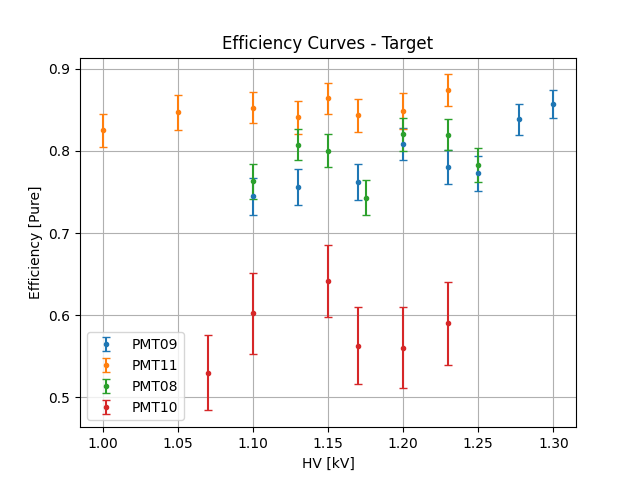
\includegraphics[width=0.5\linewidth]{Grafici/Efficiency Curves - Target.png}
    \caption{Curve di efficienza per i PMT di lettura del bersaglio}
    \label{fig:placeholder}
\end{figure}


\begin{table}[H]
    \begin{minipage}{0.45\linewidth}
        \centering
        \resizebox{1\linewidth}{!}{    \begin{tabular}{cccc}
    \toprule
    HV [V] ($\pm$ 1 V)& $\varepsilon [\%]$ & $\sigma_{\varepsilon} [\%]$ & $D_{fake}$ \\
    \midrule
    1100 & 76 & $\pm$ 2 & 0.01 \\
    1130 & 81 & $\pm$ 2 & 0.02 \\
    1150 & 80 & $\pm$ 2 & 0.02 \\
    1175 & 74 & $\pm$ 2 & 0.03 \\
    1200 & 82 & $\pm$ 2 & 0.04 \\
    1230 & 82 & $\pm$ 2 & 0.06 \\
    1250 & 78 & $\pm$ 2 & 0.07 \\
    \bottomrule
    \end{tabular}}
        \caption{PMT08}
        \label{tab:PMT08}
    \end{minipage}
    \hfill
    \begin{minipage}{0.45\linewidth}
        \centering
        \resizebox{1\linewidth}{!}{    \begin{tabular}{cccc}
    \toprule
    HV [V] ($\pm$ 1V) & $\varepsilon [\%]$ & $\sigma_{\varepsilon} [\%]$ & $D_{fake}$ \\
    \midrule
    1100 & 75 & $\pm$ 2 & 0.080 \\
    1130 & 76 & $\pm$ 2 & 0.076 \\
    1170 & 76 & $\pm$ 2 & 0.077 \\
    1200 & 81 & $\pm$ 2 & 0.077 \\
    1230 & 78 & $\pm$ 2 & 0.078 \\
    1250 & 77 & $\pm$ 2 & 0.079 \\
    1277 & 84 & $\pm$ 2 & 0.077 \\
    1300 & 86 & $\pm$ 2 & 0.079 \\
    \bottomrule
    \end{tabular}}
        \caption{PMT09}
        \label{tab:PMT09}
    \end{minipage}
    \hfill
\end{table}
\begin{table}[H]
    \begin{minipage}{0.45\linewidth}
        \centering
        \resizebox{1\linewidth}{!}{    \begin{tabular}{cccc}
    \toprule
    HV [V] ($\pm$ 1V) & $\varepsilon [\%]$ & $\sigma_{\varepsilon} [\%]$ & $D_{fake}$ \\
    \midrule
    1070 & 53 & $\pm$ 5 & 0.054 \\
    1100 & 60 & $\pm$ 5 & 0.047 \\
    1150 & 64 & $\pm$ 4 & 0.055 \\
    1170 & 56 & $\pm$ 5 & 0.054 \\
    1200 & 56 & $\pm$ 5 & 0.059 \\
    1230 & 59 & $\pm$ 5 & 0.054 \\
    \bottomrule
    \end{tabular}}
        \caption{PMT10}
        \label{tab:PMT10}
    \end{minipage}
    \hfill
    \begin{minipage}{0.45\linewidth}
        \centering
        \resizebox{1\linewidth}{!}{\begin{tabular}{cccc}
    \toprule
    HV [V] ($\pm$ 1V) & $\varepsilon [\%]$ & $\sigma_{\varepsilon} [\%]$ & $D_{fake}$ \\
    \midrule
    1100 & 74 & $\pm$ 2 & 0.077 \\
    1130 & 76 & $\pm$ 2 & 0.077 \\
    1170 & 76 & $\pm$ 2 & 0.077 \\
    1200 & 81 & $\pm$ 2 & 0.077 \\
    1230 & 78 & $\pm$ 2 & 0.077 \\
    1250 & 79 & $\pm$ 2 & 0.079 \\
    1277 & 84 & $\pm$ 2 & 0.080 \\
    1300 & 86 & $\pm$ 2 & 0.079 \\
    \bottomrule
\end{tabular}}
        \caption{PMT11}
        \label{tab:PMT11}
    \end{minipage}
    \hfill
\end{table}
\hfill
\begin{table}[H]
    \begin{minipage}{0.5\linewidth}
         Il punto di lavoro scelto è stato dunque:
    \end{minipage}
    \begin{minipage}{0.5\linewidth}
        \centering
        \resizebox{1\linewidth}{!}{\input{Tabelle/work_target}}
        \caption{Punto di lavoro scelto per il bersaglio}
        \label{tab:work_targ}              
    \end{minipage}
\end{table}


\end{flushleft}

\subsection{VETO}

\begin{flushleft}    

Infine abbiamo eseguito lo studio analogo per il PMT01(VETO). Abbiamo usato il rapporto triple su doppie della terna PMT07 - PMT09 $\vee$ PMT11 - PMT01. 

Il ragionamento per la scelta della terna di PMT è lo stesso del caso precedente del PMT10, in quanto non è presente uno scintillatore sottostante al PMT01, dunque il metodo dei trigger ortogonali non ci è risultato ottimale per la misura.

\begin{table}[H]
    \begin{minipage}{0.5\linewidth}
        \centering
        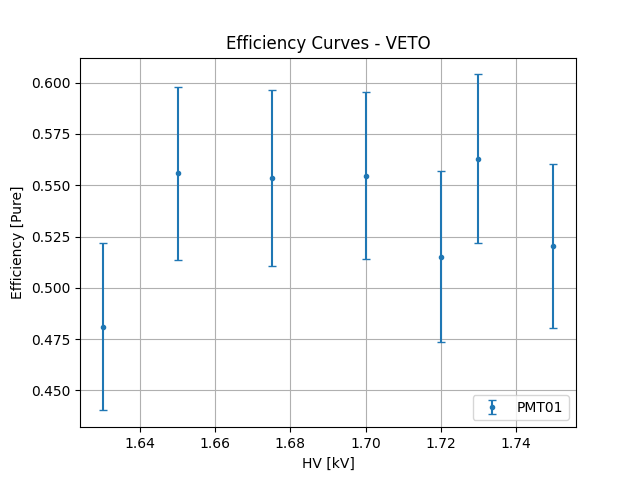
\includegraphics[width=0.91\linewidth]{Grafici/Efficiency Curves - VETO.png}
        \caption{Curva di efficienza per il PMT01(VETO)}
        \label{fig:veto_efficiency}
    \end{minipage}
    \begin{minipage}{0.5\linewidth}
        \centering
        \resizebox{0.7\linewidth}{!}{\begin{tabular}{cccc}
\toprule
HV [kV] & $\varepsilon [\%]$ & $\sigma_{\varepsilon} [\%]$ & $D_{fake}$ \\
\midrule
1.630 & 48 & $\pm$ 4 & 0.35 \\
1.650 & 56 & $\pm$ 4 & 0.35 \\
1.675 & 55 & $\pm$ 4 & 0.33 \\
1.700 & 55 & $\pm$ 4 & 0.34 \\
1.720 & 52 & $\pm$ 4 & 0.34 \\
1.730 & 56 & $\pm$ 4 & 0.33 \\
1.750 & 52 & $\pm$ 4 & 0.36 \\
\bottomrule
\end{tabular}}
        \caption{Curva di efficienza per il PMT01(VETO)}
        \label{tab:work_targ}              
    \end{minipage}
\end{table}

\end{flushleft}
\section{Presa dati}

\subsection{Logica dei segnali}
\begin{flushleft}
Per la misura del tempo di decadimento abbiamo implementato una logica di START-STOP con VETO realizzata mediante opportune combinazioni dei segnali logici discriminati\footnote{Da qui in poi ci riferiremo ai segnali dei vari PMT solamente utilizzando il loro numero in riferimento al nostro apparato come riportato in \textbf{(Metti ssezione/immagine)}.} dei vari PMT e di segnali ausiliari generati con una logica secondaria.

\begin{itemize}
    \item \textbf{VETO: $\bm{\bar{(01)}}$}, segnale proveniente dall'ultimo PMT collegato alla lastra scintillatrice più in basso, necessario per rivelare il passaggio di un raggio cosmico attraverso tutti i piani dell'apparato e di conseguenza scartare l'evento. Si utilizza  il segnale negato per necessità di logica in quanto siamo interessati a eventi di muoni che si fermano nel blocco di target;
    \item \textbf{START}: $\bm{(07\land04\land02)\land(08\lor09\lor10\lor11)\land (\bar{01})}$, La coincidenza tripla dei PMT del telescopio individua l'arrivo di un raggio cosmico, l'OR dei PMT del blocco ci dice che è passato per il blocco, mentre la coincidenza negata con il segnale di VETO rimuove eventi in cui il raggio cosmico attraverso l'apparato.
    \item \textbf{GATE}: Segnale generato con un dual timer che apre una finestra di 50$\mu \text{s}$, sul fronte di salita dello start. Necessario per filtrare a livello logico eventi indesiderati che non rappresentano decadimento del muone\footnote{la probabilità che accada dopo 20 $\mu s$ è data da \textbf{METTI CONTO}}.
    \item \textbf{STOP: $\bm{(08\lor09\lor10\lor11) \land \text{GATE} \land (\bar{01}) }$}, Segnale di OR dei vari scintillatori del blocco di target in coincidenza con il GATE per filtrare eventi indesiderati, in coincidenza con il veto per assicurarci che il segnale dal blocco di target non provenga da un cosmico che arriva in quella finestra di tempo \footnote{La probabilità che questo accada è esigua METTI CONTO ma nonostante questo abbiamo implementato ugualmente questo livello in più per essere sicuri di selezionare il più possibile solo muoni}

    
\end{itemize}

Si è inoltre dovuto regolare opportunamente le durate dei vari segnali discriminati in maniera da garantire la sovrapposizione necessaria per far si che le unità di coincidenza utilizzate generino un segnale. Allo stesso modo è necessario non estendere eccessivamente la lunghezza temporale dei segnali in qunato come si nota in \ref{fake} questa è direttamente proporzionale al rate delle coincidenze false. Di conseguenza è sembrato ragionevole per tutti i segnali dei PMT scegliere una durata di 50 ns, ad eccezione per il PMT01(VETO).
Per tale segnale è stata impostata la durata di 100 ns e anticipato di 4 ns rispetto agli altri con opportune combinazioni di cavi. 
La ragione di tale scelta è che il VETO deve bloccare l'acquisizione non appena è determinato che l'evento non corrisponde a un muone fermatosi nel blocco. Quindi vogliamo sia in anticipo per fermare subito l'acquisizione e più duraturo degli altri segnali, in modo che la coincidenza risulti eventualmente falsa per tutta la durata del segnale di START.
Per la logica scelta a ogni START corrisponde uno STOP molto ravvicinato. Si è deciso di non filtrarli via hardware, bensì di tenerne conto in sede di analisi dati in maniera da mantenere la logica semplice e avere più informazioni in sede di analisi dati.

\end{flushleft}

\subsection{Logica}

Tramite un'opportuna scelta dei segnali collegati alla scheda di sviluppo DEO10-nano sono state effettuate le prese dati necessarie alla determinazione della vita media del muone. Alla scheda sono stati quindi collegati i seguenti segnali: lo START(CH0), lo STOP(CH1) e 4 segnali aggiuntivi ottenuti dalla coincidenza del GATE con ciascuno dei PMT del blocco in OR con il negato del VETO(CH2-3-4-5).
I segnali di ogni singolo PMT del target sono stati importanti in fase di analisi dati in quanto hanno permesso di ricostruire in mainera ottimale gli intervalli di tempo e fornito informazioni sul comportamento dei singoli PMT del target.\\
L'algoritmo implementato per la ricostruzione degli intervalli di tempo ha una logica di tipo \textit{greedy pairing}\footnote{Algoritmo che una volta individuato uno Start scorre gli Stop che seguono temporalmente quest'ultimo e lo accoppiano al primo segnale di stop che rispetta una determinata condizione} in pratica:
\begin{itemize}
\item Individua uno START;
\item Controlla ci sia uno STOP, oppure uno STOP con segnale in uno dei PMT, oppure STOP con segnale in due PMT sovrapposti contemporaneamente;
\item Ripete il controllo cercando i casi precedenti o alternativamente segnale in uno dei PMT;
\item Fa la differenza fra lo START trovato all'inizio e il primo STOP utile.
\end{itemize}

\section{Analisi dati}

\subsection{Fit della vita media}

\begin{flushleft}
    
Controllando che le condizioni di lavoro dell'apparato rimanessero invariate, abbiamo effettuato diverse prese dati per massimizzare la statistica a nostra disposizione e migliorare la stima della vita media.\\
Inserisci tabella con i dati e le date dei dati.\\
Unendo i vari dataset abbiamo quindi realizzato un fit di massima likelyhood di tipo integrale ristretto agli intervalli di tempo di un certo range di valori.
La funzione utilizzata nel fit è:

\begin{equation}
    \label{fit_func}
    f(t) = Ae^{-\frac{t}{\tau}} + B
\end{equation}
Nella quale sono stati lasciati come parametri di fit $\tau$ (vita media) e $B$ (parametrizzazione del fondo presente nella nostra misura).\\

Riportiamo i risultati del fit con la distribuzione dei residui:

\begin{figure}[H]
    \centering
    \begin{minipage}{0.48\linewidth}
        \centering
        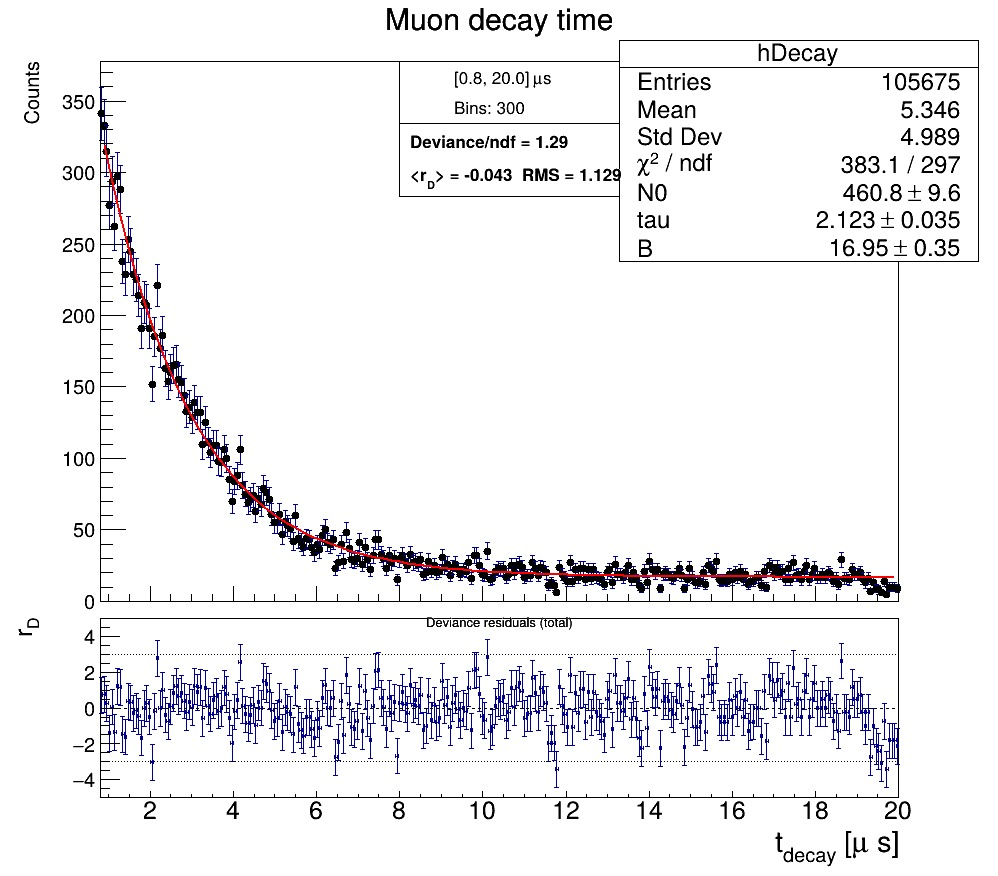
\includegraphics[width=\linewidth]{Grafici/FitFinale.jpeg}
        \caption{Risultati del fit con residui}
        \label{fig:fit}
    \end{minipage}
    \hfill
    \begin{minipage}{0.48\linewidth}
        \centering
        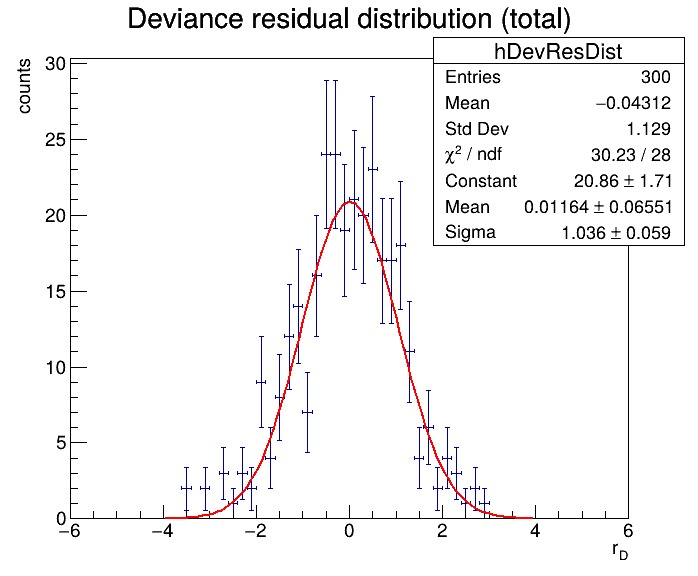
\includegraphics[width=\linewidth]{Grafici/DeistribuzioneResidui.jpeg}
        \caption{Distribuzione dei residui}
        \label{fig:residui}
    \end{minipage}
\end{figure}
%DA INSERIRE UNA PARTE SULLA QUALITà DEL FIT, COMMENTO SUI RESIDUI, INSERIRE GRAFICI PER CIASCUN PMT

Il fit restituisce un valore per vita media : $\tau = 2.123 \pm 0.035\mu$s. Questo valore è compatibile entro 2.1 barre d'errore con il valore riportato sul PDG. 

INSERISCI COMMENTO SU RESIDUI E CAZZATE VARIE.\\

\end{flushleft}
\subsubsection{Plot dei vari PMT}
INNSERISCI I PLOT\\

\subsection{Errori sistematici}
\begin{flushleft}

Abbiamo studiato la dipendenza della misura di vita media da vari parametri a nostra scelta, scrivendo un codice che realizzasse una scansione con varie combinazioni di:

\begin{itemize}
\item numero di bin $n_{bin}$
\item estremo superiore del taglio temporale ($t_{max}$)
\item estremo inferiore del taglio temporale ($t_{min}$)
\end{itemize}

Abbiamo inoltre riportato la misura in funzione del numero di scansioni.
Riportiamo dei grafici:

\begin{figure}[H]
    \centering
    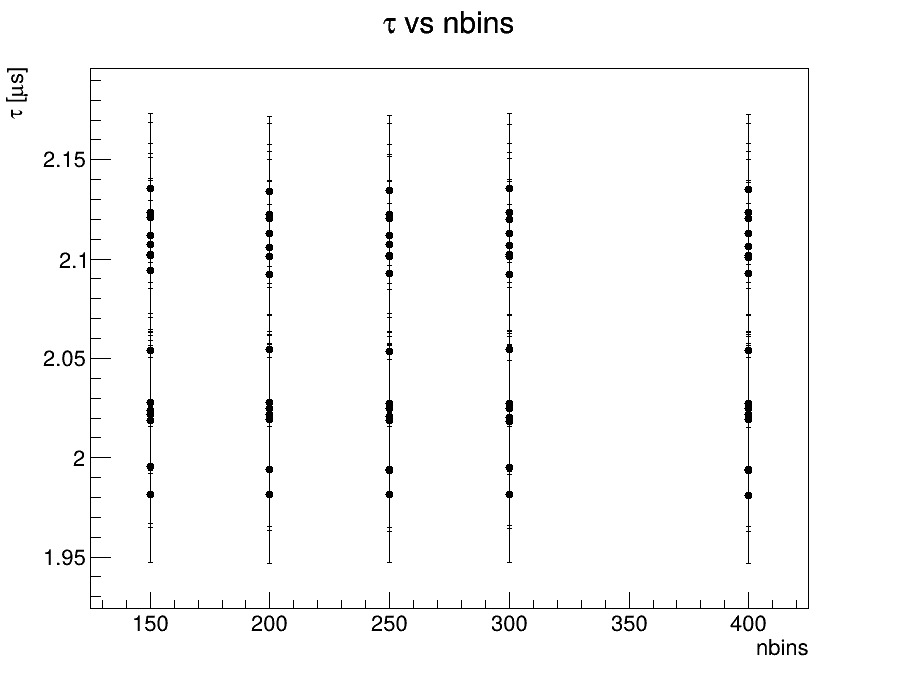
\includegraphics[width=0.5\linewidth]{Grafici/TauVSbins.jpeg}
    \caption{$\tau$ in funzione di $n_{bin}$, variando poi gli altri parametri}
    \label{fig:placeholder}
\end{figure}

\begin{figure}[H]
    \centering
    \begin{minipage}{0.48\linewidth}
        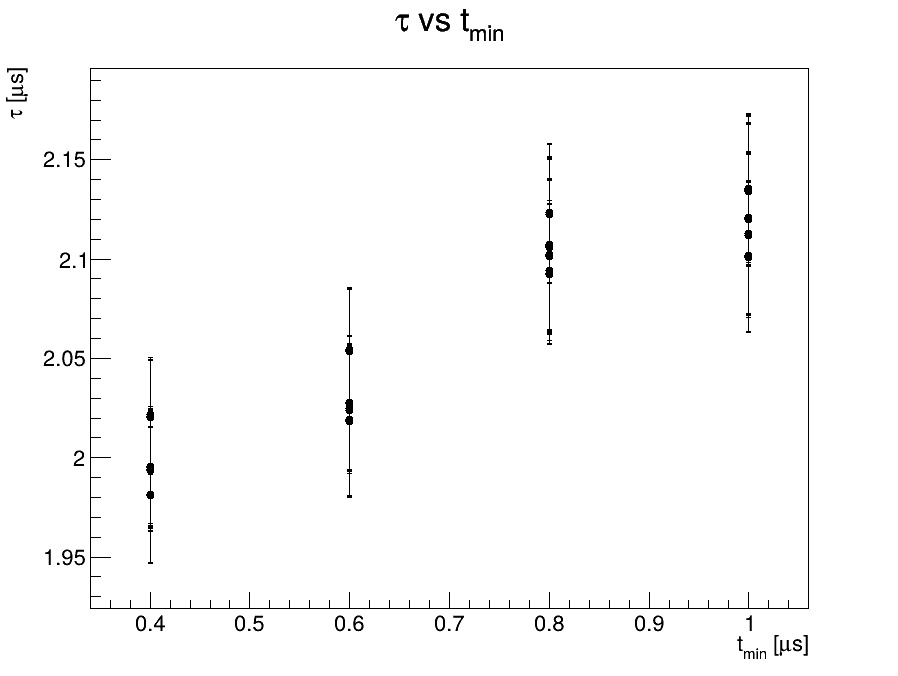
\includegraphics[width=\linewidth]{Grafici/TauVStmin.jpeg}
        \caption{$\tau$ in funzione del $t_{min}$, variando poi gli altri parametri}
        \label{fig:placeholder}
    \end{minipage}
    \hfill
    \begin{minipage}{0.48\linewidth}
        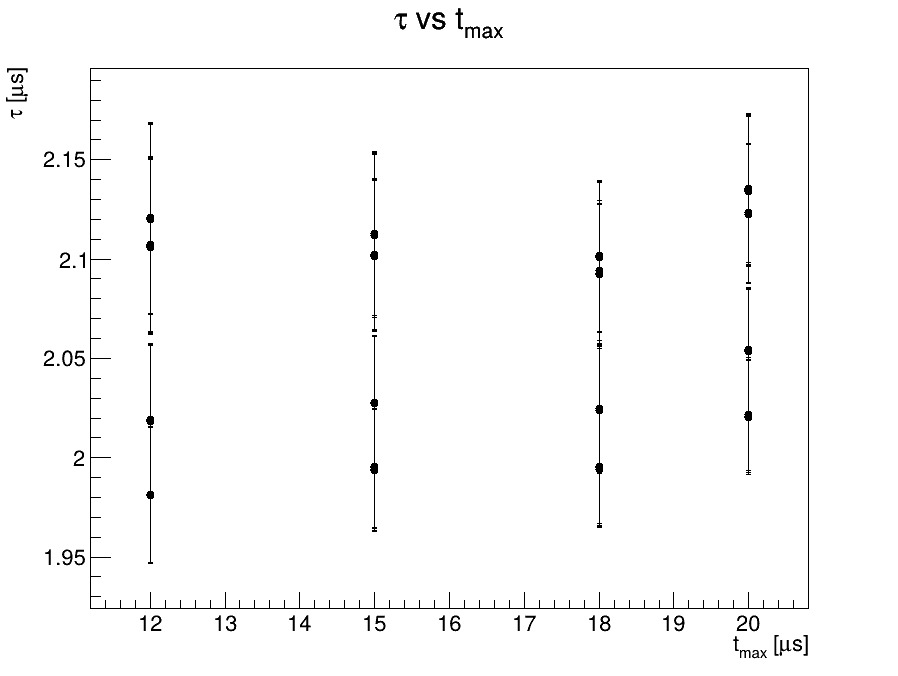
\includegraphics[width=\linewidth]{Grafici/TauVStmax.jpeg}
        \caption{$\tau$ in funzione del $t_{max}$, variando poi gli altri parametri}
        \label{fig:placeholder}
    \end{minipage}
\end{figure}
\end{flushleft}
%INSERIRE COMMENTO AI GRAFICI 
\newpage
\subsection{Misura del rapporto fra le popolazioni}
\begin{flushleft}
Abbiamo in seguito usato lo stesso set di dati per misurare l'abbondanza relativa fra muoni positivi e negativi. 

Per farlo abbiamo assunto nota la vita media del $\mu^{-}$ $\tau= 2.043\pm0.003 \mu$s, ricavando così quella per il $\mu^{+}$: 

\begin{equation}
    \label{mean_life_tot}
    \tau = \frac{1}{2}(\tau_{+}+\tau_{-}) \implies \tau_{+} = 2\tau -\tau_{-}= 2.203 \mu \text{s}
\end{equation}

Dopodiché effettuiamo un fit con la funzione:

\begin{equation}
    \label{fit_func_2}
    g(t) = A_{+}e^{-\frac{t}{\tau_+}}+A_{-}e^{-\frac{t}{\tau_-}} + B
\end{equation}

I parametri in questo caso sono $A_{\pm}$ e $B$, mentre le vite medie ($\tau_+$ e $\tau_-$) sono fissate. Definiamo quindi due funzioni esponenziali con i parametri ottenuti dal fit precedente e ne calcoliamo l'integrale. Questo sarà proporzionale al numero di decadimenti per ciascuna carica $N_{\pm}$ in queso modo possiamo ricavare il rapporto tre le abbondanze nel seguente modo:\\
\begin{minipage}{0.45\linewidth}
\centering
\begin{equation}
    \label{height_muon}
    h_{\pm}(t) = A_{\pm}e^{-\frac{t}{\tau_{\pm}}}
\end{equation}
\end{minipage}
\hfill
\begin{minipage}{0.45\linewidth}
\centering
\begin{equation}
    \label{Number_muon}
    N_{\pm} =\int _{t_{min}}^{t_{max}}  A_{\pm}e^{-\frac{t}{\tau_{\pm}}} dt
\end{equation}
\end{minipage}\\
da cui:
\begin{equation}
    \label{Abbundancies}
    R = \frac{N_+}{N_-}
\end{equation}


L'area è stata trattata come una variabile Poissoniana, di conseguenza l'errore associato a R può essere calcolato con la seguente relazione:
\begin{equation}
    \label{error_R}
    \sigma_r = R\sqrt{\frac{1}{N_+}+\frac{1}{N_-}}
\end{equation}
Utilizzando le relazioni \ref{Abbundancies} e \ref{error_R} otteniamo quindi $R = 1.07 \pm 0.08$

Il valore atteso è di 1.28 $\pm$ 0.32 (stats.) $\pm$ 0.32 (syst.), compatibile con la nostra misura.
%CITA IL CAZZO DI ARTICOLO; QUELLO DI CMS , devi inoltre mettere una stima di errore decente

\end{flushleft}
\section{Misura della massa del muone}



%DA INSERIRE I GRAFICI PER LA CALIBRAZIONE, E RIVEDI LA CALIBRAZIONE STESSA.

\subsection{Misura di spettro}
\begin{flushleft}
Per la misura di massa del muone, è necessario ricostruire lo spettro in energia dell'elettrone emesso dal decadimento e misurarne l'energia massima.
Per misurare lo spettro usiamo come trigger il segnale di STOP. Di base questo crea un problematica : infatti a ogni START corrisponde uno STOP non associato a un decadimento, dunque il segnale in uscita dall'ADC saranno due scalini che si sommano dopo un certo tempo.\\
Inserire immagini esempio delle forme d'onda digitalizzate e approfondire tutta la descrizione di cosa abbiamo osservato e digitalizzato
\\
Il primo scalino corrisponde al muone entrato nel blocco, quindi la sua altezza è proporzionale all'energia del muone. L'altezza del secondo scalino invece è proporzionale alla somma dell'energia del muone e dell'elettrone.La differenza fra l'altezza dei due scalini è dunque proporzionale all'energia dell'elettrone. 

Per ottenere il valore dell'ampiezza delle forme d'onda digitalizzate dall'adc è stato realizzato un codice di analisi dati in ROOT che esegue in breve le seguenti istruzioni:
\begin{itemize}
\item salva le forme d'onda campionate a ciascun canale, li calibra con la costante trovata e poi li somma;
\item ne fa la derivata numerica, per la forma d'onda da noi analizzata corrisponde a una gaussiana localizzata nel punto di discesa approssimabile a un impulso tanto più la discesa è rapida;
\item cerca eventi con due impulsi e ne salva le coordinate;
\item calcola l'energia come differenza fra l'altezza del secondo scalino e del primo
\item realizza un istogramma delle ampiezze.
\end{itemize}

%Riporta lo spettro, commenta e metti un immagine di un evento come esempio.
\end{flushleft}

\section{Conclusioni}
bla bla bla



\section{Bibliografia}
%\cite{ParticleDataGroup:2024cfk}
%\bibitem{ParticleDataGroup:2024cfk}
S.~Navas \textit{et al.} [Particle Data Group],
%``Review of particle physics,''
Phys. Rev. D \textbf{110} (2024) no.3, 030001
doi:10.1103/PhysRevD.110.030001
%59 citations counted in INSPIRE as of 21 Aug 2024

\newpage
\appendix
\section{Calibrazione DEO10-nano}
Per acquisire i tempi usiamo la scheda DEO10-nano. Questa prende in input (ne ha 10 in totale) i nostri segnali dopo una conversione da logica NIM a logica TTL. L'output restituito dalla scheda è un file che contiene il canale in cui c'è stato segnale e il tempo in cui tale segnale è scattato, riportato come numero di cicli di clock passati dall'inizio del conteggio. 

Per avere una misura di tempo è dunque necessaria un'opportuna calibrazione.
Per fare ciò, usiamo la funzione End Marker di un'unità di timer per mandare un segnale a una seconda, la cui uscita viene mandata di nuovo alla prima. Questo causa un auto-oscillazione che genera un'onda quadra, di parametri (frequenza e duty cycle) personalizzabili modulando la lunghezza dell'impulso.
Confrontando la lettura della scheda con la frequenza dell'onda quadra misurata all'oscilloscopio possiamo ottenere la costante di calibrazione (che corrisponde, nota bene, al periodo del clock della scheda). Svolgendo questa procedura abbiamo misurato una frequenza di 1.071 Hz.

Mandando in input l'onda quadra al NANO abbiamo acquisito dei punti e calcoliamo la differenza temporale in digit. Facendolo varie volte otteniamo una distribuzione, stimiamo dunque il periodo in digit come la media della distribuzione e l'errore associato è la deviazione standard della media. 

Per completezza abbiamo misurato anche il ritardo fra due canali (lo 0 e l'1), mandando due onde quadre in fase fra loro per vedere se vi era un ritardo dovuto all'acquisizione.

Riportiamo di seguito due grafici con le nostre misure:

\begin{figure}[H]
\centering
    \begin{minipage}{0.4\textwidth}
        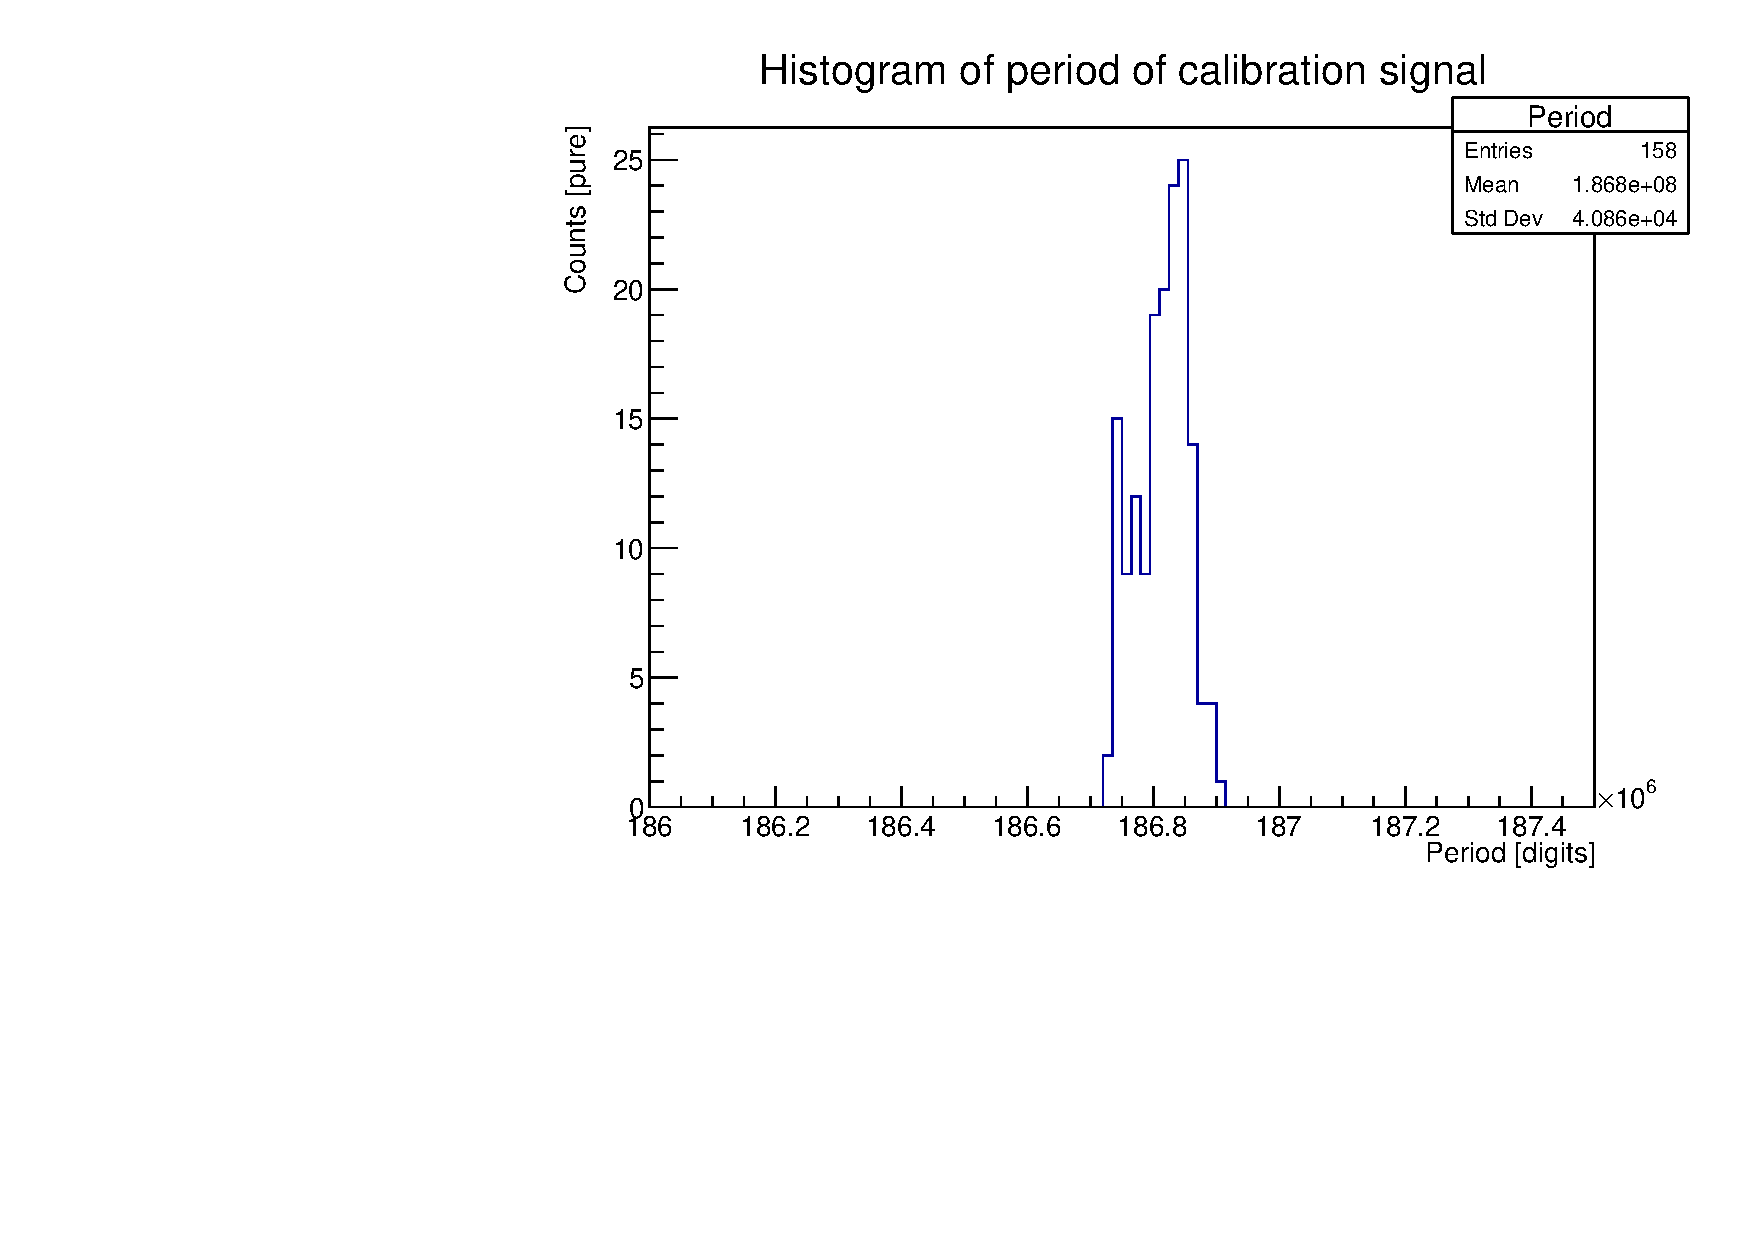
\includegraphics[width=\linewidth]{Grafici/Periodo.pdf}
        \caption{Periodi misurati per il segnale di calibrazione}
        \label{fig:placeholder}
    \end{minipage}
    \begin{minipage}{0.5\textwidth}
        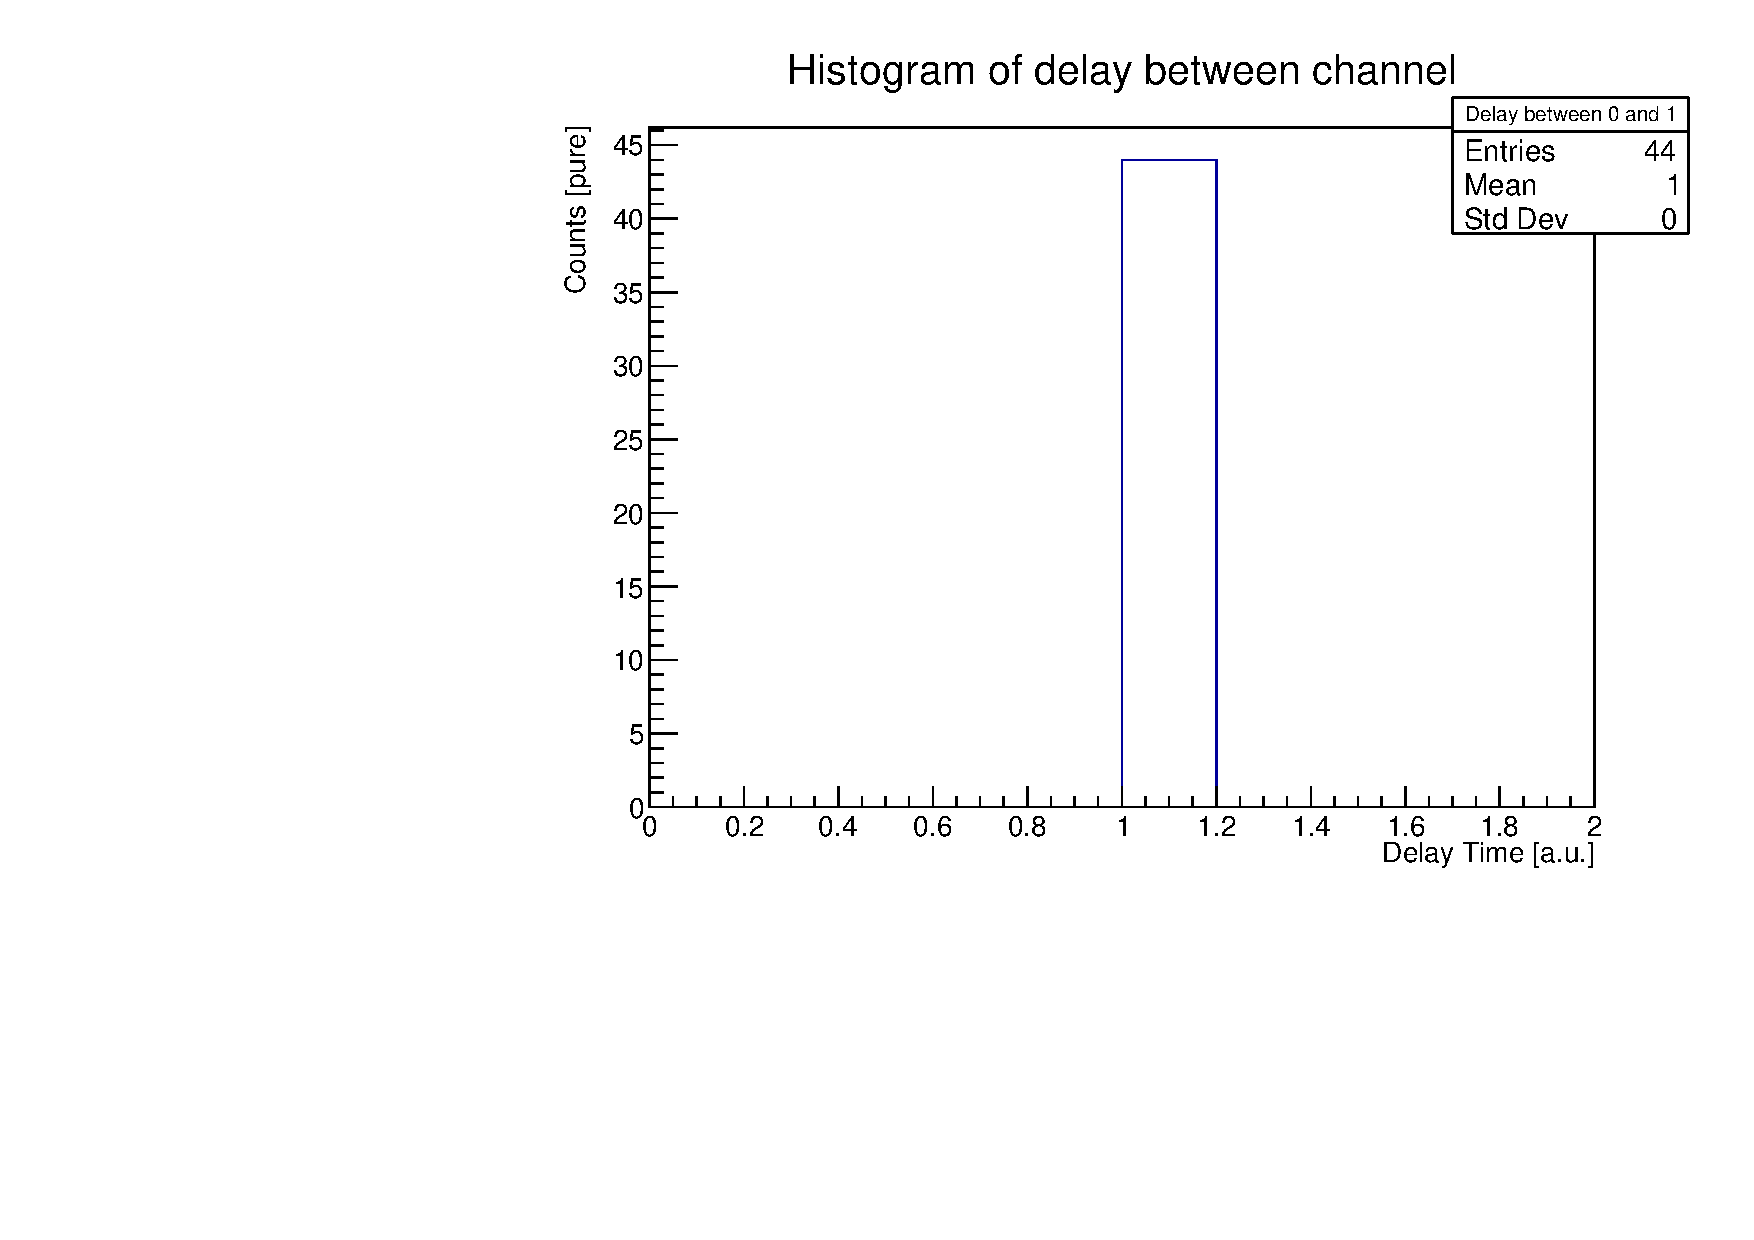
\includegraphics[width=\linewidth]{Grafici/Ritardo.pdf}
        \caption{Ritardo fra i segnali}
        \label{fig:placeholder}
    \end{minipage}
\end{figure}

Quindi, chiamata $\alpha = T[s]/T[dgt]$ la costante di calibrazione digit-tempo $\alpha = 4.98892 \pm 0.00002 $ ns/dgt. 
Il grafico a destra, d'altro canto, mostra che abbiamo un digit di differenza fra i due canali, corrispondente al valore di $\alpha$ in tempo.

\section{Calibrazione dell'ADC}
\begin{flushleft}

Utilizziamo il fatto che l'energia rilasciata nello scintillatore è proporzionale alla quantità di luce emessa, a sua volta proporzionale all'altezza dei segnali in uscita dal PMT. Necessitiamo dunque di un opportuna calibrazione, fornitaci dai raggi cosmici. 

Assumendo che essi siano MIP\footnote{Minimum Ionizing Particle: AGGIUNGI UNA BREVISSIMA DESCRIZIONE}, la loro perdita di energia è data dalla seguente relazione:
\begin{equation}
    \label{Energy_loss}
    -\frac{1}{\rho}\frac{dE}{dx} = 2\frac{MeV \cdot cm^{2}}{g} 
\end{equation}
Possiamo considerare il materiale plastico di cui è fatto il nostro scintillatore approssimabile a carbonio la cui densità è $\rho_C \simeq 1 \frac{g}{cm^{3}}$ da cui note le dimensione di ogni lastra (vedi sezione ??)  è possibile ricavare l'energia rilasciata nella lastra al passaggio della particella $\Delta E  = 60MeV$. 
Per fare in modo che l'integratore campioni i segnali corretti usiamo come segnale di trigger la coincidenza tripla:$(07\land04\land01)$, questa combinazione data la geometria dell'apparato ci assicura con ragionevole certezza che l'evento rappresenta il passaggio un raggio cosmico. 
A ciascun canale dell'integratore colleghiamo l'uscita di un PMT, che poi viene mandata a un canale dell'ADC. Calibriamo ciascun canale singolarmente, in modo da avere maggiore informazione a nostra disposizione. 
Vediamo la distribuzione delle ampiezze, rapportando il valore di energia riportato di sopra con valore medio di tale istogramma ricaviamo canale per canale la costante di calibrazione. \\
Inserisci grafico usato per la calibrazione.
\end{flushleft}



\end{document}